\documentclass[oneside,a4paper,12pt]{book}
\usepackage[american]{babel}
%\pagestyle{headings}
\frontmatter

%=============================================================================

\usepackage{amsthm}
\usepackage{xspace}
\usepackage{float}
\usepackage{ifthen}
\usepackage{amsbsy}
\usepackage{amssymb}
\usepackage{balance}
\usepackage{booktabs}
\usepackage{graphicx}
\usepackage{rotating}
\usepackage{multirow}
\usepackage{needspace}
\usepackage{microtype}
\usepackage{bold-extra}
\usepackage{geometry}
\usepackage{varioref}
\usepackage{xcolor}
\usepackage{textcomp}
\usepackage{listings}
\usepackage[normalem]{ulem} %emphasize still italic
\usepackage{ucs}
\usepackage{array}

% \usepackage[utf8]{inputenc}
% \usepackage[htt]{hyphenat}
\usepackage{times}
\usepackage{url}
\usepackage{alltt}
\usepackage{amsmath}
\usepackage{xfrac}
\usepackage{subfigure}
\usepackage{appendix}
\usepackage{stmaryrd}   % for the \shortuparrow
\usepackage[utopia]{quotchap}

\usepackage{setspace}
\usepackage[numbers, sort&compress]{natbib}
\usepackage{mdwlist}        % support for better spaced lists
% allows for temporary adjustment of side margins
\usepackage{chngpage}
\usepackage[normalem]{ulem} 

% constants

\newcounter{qcounter}

% commands
\newcommand{\n}{$\cdot$}
\newcommand{\y}{\checkmark}
\newcommand{\subscript}[1]{$_{\textrm{\footnotesize{#1}}}$}
\newcommand{\superscript}[1]{$^{\textrm{\footnotesize{#1}}}$}
\newcommand{\vertical}[1]{\raisebox{-4em}{\begin{sideways}{#1}\end{sideways}}}

\newboolean{showedits}
\setboolean{showedits}{true} % toggle to show or hide edits
\ifthenelse{\boolean{showedits}}
{
       \newcommand{\ugh}[1]{\textcolor{red}{\uwave{#1}}} % please rephrase
       \newcommand{\ins}[1]{\textcolor{blue}{\uline{#1}}} % please insert
       \newcommand{\del}[1]{\textcolor{red}{\sout{#1}}} % please delete
       \newcommand{\chg}[2]{\textcolor{red}{\sout{#1}}{\ra}\textcolor{blue}{\uline{#2}}} % please change
}{
       \newcommand{\ugh}[1]{#1} % please rephrase
       \newcommand{\ins}[1]{#1} % please insert
       \newcommand{\del}[1]{} % please delete
       \newcommand{\chg}[2]{#2}
}


% ============================================================================
% Put edit comments in a really ugly standout display

\usepackage{xcolor}
\usepackage[normalem]{ulem}
\newcommand{\ra}{$\rightarrow$}


% comments \nb{label}{color}{text}
\newboolean{showcomments}
\setboolean{showcomments}{true}
\ifthenelse{\boolean{showcomments}}
    {\newcommand{\nb}[3]{
        {\colorbox{#2}{\bfseries\sffamily\scriptsize\textcolor{white}{#1}}}
        {\textcolor{#2}{\sf\small$\blacktriangleright$\textit{#3}$\blacktriangleleft$}}}
     \newcommand{\version}{\emph{\scriptsize$-$Id$-$}}
%	 \newcommand{\ugh}[1]{\textcolor{red}{\uwave{#1}}} % please rephrase
%	 \newcommand{\ins}[1]{\textcolor{blue}{\uline{#1}}} % please insert
%	 \newcommand{\del}[1]{\textcolor{red}{\sout{#1}}} % please delete
%	 \newcommand{\chg}[2]{\textcolor{red}{\sout{#1}}{\ra}\textcolor{blue}{\uline{#2}}} % please change
	 \newcommand{\chk}[1]{\textcolor{ForestGreen}{#1}} % changed, please check
	}
    {\newcommand{\nb}[3]{}
     \newcommand{\version}{}
	\newcommand{\chk}[1]{} % changed, please check
	}

% ============================================================================
% Make quotes be italic
\renewenvironment{quote}
    {\list{}{\rightmargin\leftmargin}%
     \item\relax\begin{it}}
    {\end{it}\endlist}

\newcommand{\ttimes}{\ensuremath{\times}}

%=============================================================================

\newcommand{\needlines}[1]{\Needspace{#1\baselineskip}}

% source code
\usepackage{xcolor}
\usepackage{textcomp}
\usepackage{listings}
\definecolor{source}{gray}{0.9}
\lstset{
	language={},
	% characters
	tabsize=3,
	upquote=true,
	escapechar={!},
	keepspaces=true,
	breaklines=false,
	alsoletter={:},
	breakautoindent=true,
	columns=fullflexible,
	showstringspaces=false,
	basicstyle=\footnotesize\ttfamily,
	% background
	frame=single,
    framerule=0pt,
	backgroundcolor=\color{source},
	% numbering
	numbersep=5pt,
	numberstyle=\tiny,
	numberfirstline=true,
	% captioning
	captionpos=b,
	numberbychapter=false,
	% formatting (html)
	moredelim=[is][\textbf]{<b>}{</b>},
	moredelim=[is][\textit]{<i>}{</i>},
	moredelim=[is][\uline]{<u>}{</u>}}
\newcommand{\ct}{\lstinline[backgroundcolor=\color{white},basicstyle=\footnotesize\ttfamily]}
\newcommand{\lct}[1]{{\small\tt #1}}


%----------------------------------------------------------------------------
% references
\newcommand{\tabref}[1]{\hyperref[{tab:#1}]{Table~\ref*{tab:#1}}}
\newcommand{\figref}[1]{\hyperref[{fig:#1}]{Figure~\ref*{fig:#1}}}
\newcommand{\secref}[1]{\hyperref[{sec:#1}]{Section~\ref*{sec:#1}}}
\newcommand{\lstref}[1]{\hyperref[{lst:#1}]{Listing~\ref*{lst:#1}}}
\newcommand{\charef}[1]{\hyperref[{cha:#1}]{Chapter~\ref*{cha:#1}}}
%----------------------------------------------------------------------------

% abbreviations
\tracingcolors 4
\setcounter{tocdepth}{3}
\setcounter{secnumdepth}{3}
\newcommand{\ie}{\emph{i.e.,}\xspace}
\newcommand{\eg}{\emph{e.g.,}\xspace}
\newcommand{\etc}{\emph{etc.}\xspace}
\newcommand{\etal}{\emph{et al.}\xspace}


\newcommand{\newevenside}{
	\ifthenelse{\isodd{\thepage}}{\newpage}{
	\newpage
        \phantom{placeholder} % doesn't appear on page
	\thispagestyle{empty} % if want no header/footer
	\newpage
	}
}

\def\stretchfactor{1}
\newcommand{\mychapter}[1]{\setstretch{1}
    \chapter{#1}\setstretch{\stretchfactor}}

%----------------------------------------------------------------------------
\newcommand{\lessSpace}{\vspace{-1em}}
\DeclareGraphicsExtensions{.pdf,.png}
\graphicspath{{images/}}
\newcommand{\fig}[4]{
	\begin{figure}[#1]
		\centering
		\includegraphics[width=#2\textwidth]{#3}
		\lessSpace
		\caption{\label{fig:#3}#4}
	\end{figure}}

% ===========================================================================

%:CONFIGURE THIS

\newcommand{\thesistitle}{Cryptographic APIs}
\newcommand{\thesisauthor}{Sophie Gabriela Pfister}
\newcommand{\thesisauthorOrigin}{Bern, Switzerland}
\newcommand{\thesisleiter}{Prof.\ Dr.\ Oscar Nierstrasz}
\newcommand{\thesisasst}{Dr.\ Mohammad Ghafari, Mohammadreza Hazhirpasand}
\newcommand{\thesisurl}{http://scg.unibe.ch/}
\newcommand{\thesissubtitle}{Evaluating the Usability of Java Cryptography Architecture}
\newcommand{\thesisdate}{31. Dezember 2021}

% ===========================================================================

\usepackage[ colorlinks=true, urlcolor=black, linkcolor=black,
			citecolor=black, bookmarksnumbered=true, bookmarks=true,
			plainpages=false,
			pdftitle={\thesistitle}, pdfauthor={\thesisauthor},
			pdfsubject={\thesissubtitle}, pdfpagelabels]{hyperref}

\newcommand{\hrref}[2]{\hyperref}
% ===========================================================================
% ===========================================================================

\hypersetup{
    colorlinks=true,
    linkcolor=black,
    filecolor=magenta,      
    urlcolor=blue,
    }

% D O C U M E N T
% % % % % % % % % % % % % % % % % % % % % % % % % % % % % % % % % %
\begin{document}

% T I T L E
% % % % % % % % % % % % % % % % % % % % % % % % % % % % % % % % % %
\begin{titlepage}  
  \begin{center}  
  
  \begin{figure}[t]  
  \vspace*{-2cm}        % to move header logo at the top 
  \center{
\includegraphics[scale=0.5]{logos/UNI_Bern.png}}
  \vspace{1.2in}     
  \end{figure}

    \thispagestyle{empty}
    
    {\bfseries\Huge \thesistitle \par
    \Large \vspace{0.1in} \thesissubtitle \par}

    \vspace{0.3in} 
    \LARGE{\textbf{Bachelor Thesis} \\}
    \vspace{0.4in}

    {\Large \thesisauthor \par from \par \thesisauthorOrigin}
    
    \vspace{0.3in}
    {\Large Philosophisch-naturwissenschaftlichen Fakult\"{a}t \\
            der Universit\"{a}t Bern \par}
    \vspace{0.3in}
    {\Large \thesisdate \par}
    \vspace{0.3in}
    %Leiter der Arbeit: \par
   {\Large \thesisleiter} \par
      {\Large \thesisasst} \par
   \vspace{0.1in}
    {\Large Software Composition Group \par Institut f\"{u}r Informatik \par University of Bern, Switzerland \par}
  

  %\vspace{0.5in}
 
 

  \end{center}

\end{titlepage}


% A B S T R A C T
% % % % % % % % % % % % % % % % % % % % % % % % % % % % % % % % % %
\chapter*{\centering Abstract}
\begin{quotation}
\noindent 
% ToDo: Abstract
\end{quotation}
\clearpage


% C O N T E N T S 
% % % % % % % % % % % % % % % % % % % % % % % % % % % % % % % % % % % % % % % %
\tableofcontents

\mainmatter
%%%%%%%%%%%%%%%%%%%%%%%%%%%%%%%%%%
%%%% NEW CHAPTER %%%%%%%%%%%%%%%%%%%%%
%%%%%%%%%%%%%%%%%%%%%%%%%%%%%%%%%%

% === I N T R O D U C T I O N ===
\chapter{Introduction}
\label{cha:Introduction}
% === Relevance of Cryptography  & Cryptographic APIs + Issues ===
Cryptography is a fundamental part of our digital world. 
It provides techniques to ensure confidentiality, authenticity, and integrity of information. 
Yet, Buchanan \cite{buchanan2017} describes the internet as an unsafe place. 
He complains that too little security is implemented in the services and protocols used. 
He insists that "the next generation of the Internet [...] must be built in a trustworthy way" (Buchanan, 2017, \cite{buchanan2017}, p. 1).\\
At first sight, this statement seems surprising, since there are cryptography libraries for all common programming languages. 
They support developers building secure applications by providing services such as hashing, message authentication, symmetric, and asymmetric encryption.
However, past research revealed that software developers are struggling to make use of them.
They often lack \emph{usability}. 
As you will see in chapter \ref{cha:CryptoApi}, this can be observed for a wide range of cryptography libraries and programming languages.
The results of Acar \etal \cite{acar2017} imply that unusable cryptography libraries do not only prevent developers from writing functioning code but also lead to security vulnerabilities as programmers are more likely to misuse them.\\
% === Relevance of Documentation for Usabilty
\par
The usability of an API depends on many aspects that influence each other (see chapter \ref{cha:ApiUsability}).
The easiest way to increase an existing API's usability is probably improving documentation quality.
It can be modified without the risk that working applications break.
Additionally, a good documentation is a strong predictor for both, functioning and secure code.
Acar \etal emphasize "the importance of creating official documentation that is useful enough to keep developers from searching out unvetted, potentially insecure alternatives" (2017, \cite{acar2017}, p. 167).\\
% === Project Goals & Research Questions ===
\par
Within the context of API usability, documentation usability, API misuse and unsafe code, we investigated to following research questions:
\begin{enumerate}
	\item What issues do programmers face when implementing symmetric encryption using Java Cryptography Architecture?
	\item What security risks can be found in code and advises shared on Stack Overflow referring to the implementation of symmetric encryption scenarios Java Cryptography Architecture?
	\item To what extent are these issues linked to missing or inadequate documentation?
\end{enumerate}
We focused on one library and one use case to gain a deeper understanding of the issues than previous research that analyzed the libraries on a more general level.
The decision for the Java Cryptography Architecture (JCA) library and the use case of symmetric encryption was based on the findings by Nadi \etal \cite{nadi2016} from 2016. 
They investigated the issues Java developers face when implementing cryptography tasks.
According to their result, JCA is the most popular cryptography library for Java and symmetric encryption is the most common cryptography task.
Also, JCA acquired FIPS-140 standards issued by NIST \footnote{National Institute of Standards and Technology} to specify the requirements for cryptography libraries and modules \footnote{\href{https://nvlpubs.nist.gov/nistpubs/FIPS/NIST.FIPS.140-3.pdf}{FIPS-140-3}}.\\
% === Methodology ===
\par
To answer our research questions, we analyzed 150 threads from Stack Overflow containing issues related to our scope.
We identified the issues as well as potential security risks and derived a set of questions that these issues relate to.
Afterwards, we sought the answer in the documentation.\\

% === Thesis Structure ===
% ToDo
\par
This thesis first presents the state of research in the related work chapter. 
The third chapter then describes the methodical approach of our study more precisely. 
You can find the results as well as their interpretation in the fourth chapter.
The fifth chapter includes the conclusion as well as conductive thoughts.
In the "Anleitung zum Wissenschaftlichen Arbeiten" (chapter six), you can learn more about Mayring's guidelines for qualitative content analysis that were followed during our analyses.

% === T H E O R Y   &   R E L A T E D   W O R K ===
\chapter {Theoretical Background and Related Work}
\label{cha:Theory}

% === Usability ===
\section{API Usability}
\label{cha:ApiUsability}
ISO 92411-11:1998 defines usability as "the extent to which a product can be used by specified users to achieve specified goals with effectiveness, efficiency and satisfaction in a specified context of use" (ISO 9241-11, \cite{iso1998}, p.2).
Although this definition is very precise, it is not specific.
It therefore does not tell us how to measure usability nor does it help us to determine whether a product is usable or not.\\
\par
Past research on API usability approached the topic in different ways.
The literature about API usability is therefore rather heterogeneous.
While some researchers defined metrics, guidelines and heuristics, others focused on the concept of usability and tried to expand it such that it meets the requirements of the domain.
Mosquiera-Rey \etal \cite{mosqueira2018} combined these approaches by extending the  usability model elaborated by Alonso-Ríos \etal \cite{alonso2010} with a contextual dimension and mapping existing guidelines to the model's categories.
They ended up with a total of 45 heuristics belonging to 9 different main aspects of usability.
\begin{figure}[h]
\centering
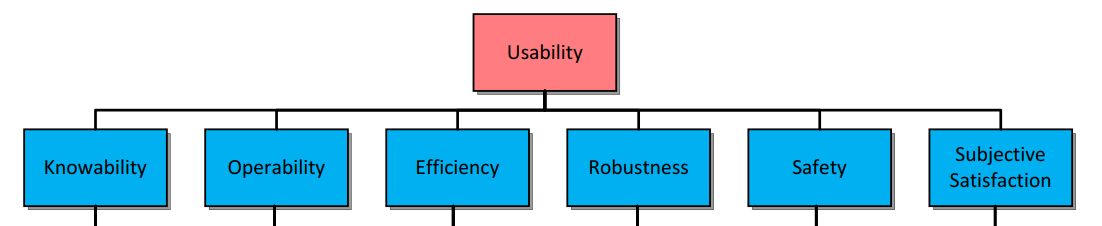
\includegraphics[width=0.65\textwidth]{ApiUsability}
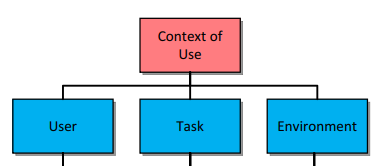
\includegraphics[width=0.33\textwidth]{ContextOfUse}
\caption{First Level of Usability and Context of Use Taxonomies (Mosquiera-Rey \etal, 2018, \cite{mosqueira2018}, p. 49 ff.)}
\label{fig:ApiUsability}
\end{figure}
\newpage
\par
This example is only supposed to illustrate the complexity of the domain. 
In the following section, we are focusing on the usability of documentation as this is what we are investigating in this thesis.

% Documentation Usability
\subsection{Usability Criteria for Documentation}
According to Mosquiera-Rey \etal \cite{mosqueira2018}, documentation has an influence on the \emph{Knowability} of an API.
This property indicates to what extent a programmer can "understand, learn, and remember how to use the system" (Mosquiera-Rey \etal, 2018, \cite{mosqueira2018}, p. 48).
One heuristic says that the documentation should not contain irrelevant information such as meta data or obsolete and redundant comments.
However, it "should include code samples for the most common scenarios"  (Mosquiera-Rey \etal, 2018, \cite{mosqueira2018}, p. 55) as well as tutorials on how to use the API.
It also should identify deprecated methods, explain why these are deprecated, and propose alternatives.
Another heuristic that is indirectly related to documentation says that "names should be self-explanatory" (Mosquiera-Rey \etal, 2018, \cite{mosqueira2018}, p. 55).
The programmer should not have to look at the documentation to understand what a function does.\\

\par
\colorbox{yellow}{ToDo}

% Crypto API Usability
\section{Usability of Cryptography Libraries}
\label{cha:CryptoApi}
In 2016, Green \& Smith \cite{green2016}



\section{Misuse of Cryptography Libraries}






% === M E T H O D O L O G Y ===
\chapter {Methodology}
\label{cha:Methods}
To answer our research questions, we first had to identify the issues programmers face when implementing symmetric encryption using JCA.
We derived them by analyzing 150 threads on Stack Overflow which is one of the most popular Q\&A forums for programmers.
We also scanned those threads regarding security risks.
We then reprocessed the results to define a set of questions that should be answered in the documentation.
Finally, we checked the documentation to see whether those questions are answered or not.\\

\par
As we required several methodical approaches, this chapter is divided into five sections.
The first section describes the sampling process.
The second section refers to identifying issues from Stack Overflow posts.
The third section explains how we checked the threads for security issues.
The fourth and last section is about the analysis of the library's documentation.\\

\newpage
% === Sampling ===
\section{Sampling}
\label{cha:MetSampling}
In JCA, symmetric encryption is implemented using the \lstinline|Cipher| class.
It supports a wide range of symmetric and asymmetric encryption algorithms.
To search for suitable threads on Stack Overflow, we first defined a set of queries.
We use the \lstinline|[java]| tag combined with a minimal \lstinline|Cipher.getInstance()| statement for each symmetric algorithm.
This statement must be executed in all encryption scenarios using \lstinline|Cipher| class.\\
As some of the symmetric algorithms supported by JCA are not very popular, the corresponding queries returned only a small amount of posts.
We decided to exclude those algorithms and focused on the three most popular symmetric encryption algorithms: AES, DESede and DES.\\
\par
Next, we calculated the sampling size using the \href{https://www.surveymonkey.com/mp/sample-size-calculator/}{sample size calculator by SurveyMonkey}.
To ensure a confidence level of 95\% and a margin of error below 8\%, we required 150 posts.
Then, we computed sample size per query proportionally to the number of posts a it returns.
The result can be found in table \ref{tab:SampleSize}.

%=== Do Not Change This Table! ===
\begin{center}
\begin{table}[h]
% === Sampling Sizes JCA
\begin{tabular}{|m{8cm}|m{2cm}|m{3cm}|}
\hline
\textbf{Query} & \textbf{\#Posts} & \textbf{Sample Size} \\
\hline
\lstinline|[java] Cipher.getInstance(AES)|&3233&126\\
\hline
\lstinline|[java] Cipher.getInstance(DESede)|&295&12\\
\hline
\lstinline|[java]Cipher.getInstance(DES) --DESede|&300&12\\
\hline
\end{tabular}
\caption{Computation of Sample Sizes}
\label{tab:SampleSize}
\end{table}
\end{center}
%=======================================
\par
Finally, we selected the threads.
We picked half of the sample from the newest\footnote{based on the creation date of the question} threads and the other half from the most popular\footnote{based on the view count} ones.
This approach attempts to balance the ambition to detect present issues with the fact that most programmers first search for answers on Stack Overflow (generating views) before posting a question.\\
As the aim of the analysis was to reveal issues referring to the implementation of \emph{symmetric encryption} using the \emph{JCA} library, we excluded all posts that did not refer to this scope.
Of course it is possible that several issues are discussed in one thread.
A thread was included if at least one issue, question, or advise referred to our scope.

\newpage
% === Analysis 1 ===
\section{Analysis of Issues}
\label{cha:MetIssues}
The goal of the first analysis was to answer the first research question: \emph{What issues do programmers face when implementing symmetric encryption using Java Cryptography Architecture?}
We followed the guidelines for qualitative content analysis by Mayring \cite{mayring2015}. 
They are a standard in humanities to evaluate text-based data and are especially well suited for method-integrative approaches that combine qualitative and quantitative elements.
They allow to evaluate large amounts of material and quantify individual analysis steps - which is exactly what we need to answer our first research question.
They also provide a set of criteria to evaluate the validity and reliability of a methodical approach.\\
In this section, we will only provide the information to understand the process. You can find the complete processing scheme in the "Anleitung zu Wissenschaftlichen Arbeiten", chapter \ref{cha:AWI}.\\
\par
We conducted the analysis in three rounds.
We first applied \emph{summarizing} to extract the relevant information (issues and questions) from the threads.
Then we classified the issues in two rounds.\\

% === Summarizing ===
\subsection{Summarizing}
The goal of this first analysis step was to extract all relevant information and record it such that we did not have to re-read the entire threads during further evaluation.
We considered the question post, posts marked as "accepted answers" as well as comments to those posts.
If there was not any accepted answer, we considered all posts and comments and tried to display the discussion in our records.\\
We conducted summarizing first on our own and discussed the results afterwards to create a consistent and more objective list of records.
In particular, we eliminated records that did not refer to our scope.
As an example, we excluded all issues that referred to the conversion of plain text or the cipher text as data conversion (or character encoding) is not only required in the context of cryptography.
\par
For each thread, we recorded the set of issues and questions that the person writing the question post (\emph{original poster}) was facing.
Then we tried to identify the reasons and solutions or answers.
We aimed for a short issue description (e.g. an error message or a shortened form of a question) and more precise explanations for the reasons and solutions.
To stay as near to the material as possible, we copy-pasted words, sentences or even paragraphs.\\

\newpage
% === Classification ===
\subsection{Classification}
As already mentioned, we classified the threads in two rounds regarding two different kind of aspects. 
We first classified all records regarding technical aspects and then classified the records regarding requirements the person asking the question was not able to meet.
In each round, we assigned at most one category to a record.
We also wanted to assign at least one category to each record.
So in the end, a record should have one or two assigned categories.

% Technical Aspects / Implementation
\subsubsection*{Technical Aspects}
In the first round of classification, we focused on the technical aspects of implementing symmetric encryption.
As categories, we defined a set of tasks that programmers must take care of when implementing symmetric encryption using JCA.
If they implement all tasks correctly, the code compiles and runs without rising an error and leads to the expected result.
So if programmers ask questions on Stack Overflow about a technical aspect, they either implemented a task incorrectly or they have a question regarding one of these tasks. 
In this classification we asked 
"What implementation step was performed incorrectly causing the error?" or 
"What implementation step is targeted by the question?".\\

Identifying a set of main tasks was simple: \emph{Cipher Object Instantiation, Generating Algorithm Parameters, Cipher Object Initialization, Transformation, and Transmitting Algorithm Parameters}.
But as we wanted to have more insight, we also defined subcategories.
To do so, we consulted the "Java Cryptography Architecture (JCA) Reference Guide" \cite{javaReferenceGuide} which provides code examples as well as explications regarding the use of the different APIs.
To allow an unambiguous category assignment, we also defined the dependencies as categories.
As a result, the following technical categories and subcategories were derived:
\begin{itemize}
	\item \textit{Cipher Object Instantiation}:
				We assigned this category to all issues and questions referring to an inappropriate \lstinline|Cipher.getInstance(...)| statement.
				As parameter, programmers must pass a transformation string consisting of:
				\begin{itemize}
					\item \textbf{Algorithm} (mandatory)
					\item \textbf{Encryption Mode} (optional)
					\item \textbf{Padding Mode} (optional)
				\end{itemize}
				Additionally, we defined the following subcategories:
				\begin{itemize}
					\item \textbf{Dependency Encryption Mode - Padding}: The encryption modes determines whether padding is required or not.
								We assigned this category to all issues caused by an inappropriate specification of those two properties.
					\item \textbf{Cipher Object Instantiation - Other} for issues and questions related to \lstinline|Cipher| object instantiation but not any of the aforementioned aspects.
				\end{itemize}
	\item \textit{Generating Algorithm Parameters}: 
				Depending on the specification of the cipher object, it requires different kind of parameters. 
				For encryption, the programmer might need to perform the following tasks:
				\begin{itemize}
					\item \textbf{Key Derivation} for issues and questions referring to random key generation, password based key derivation or key exchange protocols.
					\item \textbf{Initialization Vector / Nonce Generation} for issues and questions referring to the generation of the IV or nonce used for the transformation.
					\item \textbf{Generation of Other Algorithm Parameters}, e.g. a \lstinline|GCMParameterSpec| object which contains additional parameters for GCM encryption mode.
				\end{itemize}
	\item \textit{Cipher Object Initialization}: We assigned this category to all issues caused by the misuse of the \lstinline|init(...)| statement, e.g. not passing all required
						parameters. We defined the following subcategories:
				\begin{itemize}
					\item \textbf{Dependency Algorithm - Key}: The algorithm determines what data type the key must be stored in. 
									It also defines the allowed key sizes.
									We assigned this category to issues caused by passing an inappropriate key to the \lstinline|init(...)| method or questions about this dependency.
					\item \textbf{Dependency Algorithm \& Encryption Mode - IV}: The encryption mode determines, whether an IV is required or not.
									For some encryption modes (e.g. "CBC") the IV must be the same size as the algorithms block size.
									As an example, an issue related to passing an IV of the wrong size to the \lstinline|init(...)| method was assigned to this category.
					\item \textbf{Cipher Object Initialization - Other}
				\end{itemize}
	\item \textit{\textbf{Transformation}}: This category was assigned to all issues and questions targeting the actual transformation methods \lstinline|update(...)| and \lstinline|doFinal(...)|, e.g. passing the wrong input parameters or questions about the output.
	\item \textit{Transmission of Parameters}:
				As all parameters from encryption must be reused for decryption, they must either be stored or transmitted. 
				This category was assigned to all issues and questions referring to storing, restoring, or transmitting parameters.
				We defined the following subcategories:
				\begin{itemize}
					\item \textbf{Key Transmission}: The key must be kept secret.
					\item \textbf{Transmission of Other Parameters} such as the initialization vector. 
						They can be transmitted along the cipher text as they do not have to remain secret.
	 			\end{itemize}
	\item \textbf{Dependency Encryptor - Decryptor}: 
				The \lstinline|Cipher| objects used for encryption and decryption must be specified and initiated in the exact same way except for the parameter specifying the operation in the \lstinline|init(...)| statement.
				We assigned this category to all issues caused by differing configurations.
\end{itemize}
You can find a list with concrete examples for each category in the appendix.\\ %ToDo

% Implications / Requirements
\subsubsection*{Requirements}
As the first set of categories only targeted the implementation of symmetric encryption, we defined a second set of categories regarding the design of an application.
We defined different kind of functional and non-functional requirements as categories.
We consulted  Sommerville \cite{sommerville2011} as a theoretical basis.
During the analysis we asked ourselves "Which requirements are not met?".
Not all requirements defined by Sommerville occurred in our analysis.
We only assigned the following categories:
\begin{itemize}
	\item \textbf{Functional Requirements} to issues where a programmer was not able to fulfill a certain requirement or tried to use encryption for an unsuitable use case.
	\item \textbf{Performance} to issues where an implementation was not as time-efficient as required.
	\item \textbf{Space} to code leading to an \lstinline|OutOfMemoryException|.
	\item \textbf{Reliability} to situations where the implementation crashed frequently.
	\item \textbf{Portability} to implementations that behaved differently on different (Java) plattforms.
	\item \textbf{Interoperability} to issues where a developer was not able to decrypt a cipher text that was produced using another library or vice versa.
	\item \textbf{Security} to implementations containing security risks.
\end{itemize}
\par
As we analyzed the discussion, we only assigned a category if either the person asking the question complained about not being able to meet a certain requirement or someone gave a hint.
We conducted a broader examination of security risks in our second analysis (see chapter \ref{cha:MetSec}). 


% Evaluation
\subsection{Evaluation} % ToDo
We conducted several forms of frequency analysis' on our data.
We computed the absolute and relative frequencies for each category and subcategory.
Finally, we also took a look at the combination of technical aspects and requirements categories.
In our interpretation, we focused on the most occurring categories as these refer to more prevalent issues.\\
\colorbox{yellow}{ToDo}

% === Analysis 2 ===
\section{Analysis of Security Risks}
\label{cha:MetSec}
The goal of this second analysis was to answer the second research question: 
\emph{What are common security risks in code and advises shared on Stack Overflow referring to the implementation of symmetric encryption scenarios Java Cryptography Architecture?}\\
We first defined a set of security rules regarding the implementation of symmetric encryption.
Then we reprocessed the original sample checking them for rule violations.

\subsection{Security Rules}
We derived our rules from the rule sets used for CRYLOGGER tool (see Piccolboni \etal \cite{piccolboni2020}) and the CrySL based compiler for Java applications by Krüger \etal \cite{kruger2019}.
We only considered the rules that were applicable to symmetric encryption and structured them using the categories from technical aspect's classification (see section \ref{cha:MetIssues}).
We also abstracted the context of the rules to facilitate their evaluation.
As an example, R-04 of CRYLOGGER says " Don’t use the operation mode CBC (client/server scenarios)" (Piccolboni \etal, 2020, \cite{piccolboni2020}, p.5).
We abstracted the context and defined that a programmer should not use CBC at all.
We often do not know in what context the original poster wanted to use the code.
Additionally, if we think about someone naively copy-pasting code from Stack Overflow, the use of CBC is a potential security risk.\\
The resulting rules can be found in table \ref{tab:Rules},

\subsection{Tracking Security Rule Violations}
We reprocessed the original sample marking for each rule whether it was violated or not.
We only considered the question post, the accepted answer post, and comments to one of these.
We also distinguished between "question" and "answer" as well as "code" and "text".
We analyzed the four aspects independently and made a list for each one of them:
\begin{itemize}
	\item \textbf{Question Code} to track security risks in code snippets of the question post
 	\item \textbf{Question Text} to track security risks in the text of the question post as well as comments to it by the original poster
	\item \textbf{Answer Code} to track security risks in code snippets of the answer post
	\item \textbf{Answer Text} to track security risks in the text of the answer post as well as any comment by another person.
\end{itemize}
While analyzing the code snippets, we focused on the parts where encryption, decryption, key derivation, IV generation, and key storage were implemented.
As an example, if someone is defining a static key in the main method and passes it to the encryption section as a parameter, we did not consider this a security risk.
The encryption section can still be safe if an appropriately derived key is passed.\\
The answers were only analyzed if there was an accepted one.\\
\begin{table}[h]
\centering
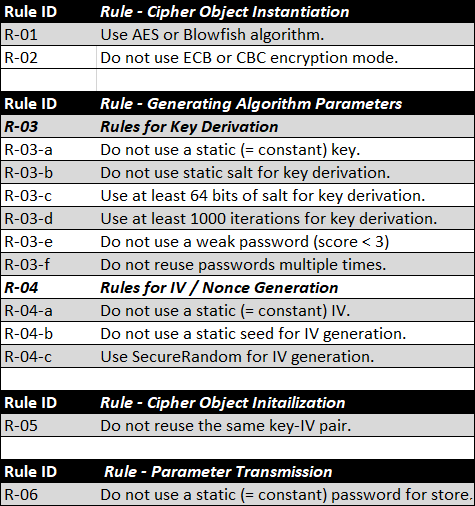
\includegraphics[width=0.7\textwidth]{Rules}
\caption{Security Rules}
\label{tab:Rules}
\end{table}

\subsection{Evaluation}
We conducted a frequency analysis for each list.
Our aim was to find out the most prevalent security risks to answer the research question. \colorbox{yellow}{ToDo}\\


% === Analysis 3: Documentation ===
\section{Analysis of Documentation}
\label{cha:MetDoc}
The results from the precedent analyses formed the basis to analyze the documentation for JCA.
As it spreads over several documents and sources, we only examined the most basic ones:
the Java Cryptography Architecture (JCA) Reference Guide \cite{javaReferenceGuide}, 
the Java Security Standard Algorithm Name Specification \cite{javaStandardAlgorithmName}, 
and the entire API documentation for \lstinline|javax.crypto| package starting from the package overview \cite{javaxCrypto}.
These three documents are valid for all providers and therefore apply to a wide range of platforms.\\
\par
To analyze the documentation, we first defined a set of question that should be answered.
Afterwards, we sought the answers in the documentation.
Our aim was to answer the third research question: 
\emph{To what extent are those issues\footnote{obstacles in implementation, security risks in code} linked to missing or inadequate documentation?}
The questions additionally gave us more insight in what programmers are struggling with.
They helped us to answer then first research question more precisely.

\subsection{Deriving Questions}
As an API documentation should support the usage of the API and not educate the programmer, basic questions regarding cryptography should not be answered in it.
However, a cryptography API should link reliable sources. %ToDo: Find reference!
We therefore created two lists of prioritized questions: one with "questions to documentation" and one containing "general questions".\\
\par
We derived the questions from the results of the former analyses.
We reprocessed the records from the first analysis and tried to formulate a question for each one.
If the question was new, we wrote it down and set its priority to one.
If there was already a similar question, we increased its priority by one and sometimes reformulated the question.\\
The set of questions derived from the first analysis' results covered already a wide range of security related topics.
We therefore did not have to add more questions based on the second analysis' findings.
However, we adapted the priorities of those questions, setting them to the actual number of threads that included a related security risk.

\subsection{Consulting Documentation}
For each question on the list, we then tried to find an answer in the documentation.
Depending on the question, we checked the different sources in another order.
We aimed to find answers as efficiently as possible.\\
For "questions to documentation", we typically started with the reference guide to find general explanations and then consulted the related parts of the API documentation.
For "general questions" we started in the standard algorithm name specification.
Of course, we knew the documentation better after answering a set of questions and therefore optimized our search strategies.\\
Once we found an answer to the question, we recorded its source as well as some remarks regarding documentation quality.

% === Evaluation ===
\subsection{Evaluation}
We first wanted to find out, what percentage of questions remained unanswered.
This gave us a starting point to answer the research question.
If most questions are answered in a clear way, we cannot blame the documentation for the issues programmers face during implementation.
We also cannot blame it for unsafe code if it contains enough hints and advises regarding security.\\
In the further evaluation we focused on the unanswered questions and our comments regarding documentation quality to make suggestions regarding the improvement of the documentation.\\
We also had a closer look at the questions as they gave us more insight regarding the first research question.\\



% === R E S U L T S ===
\chapter {Results and Interpretation}
\label{cha:Results}
In this chapter, we discuss the results of our three analyses and their interpretation.
There is a section for each of the three conducted analyses:
The first section shows the issues and the second section the security risks we found in our sample data.
The third section explains how the previous findings are linked to the documentation.\\


% === Issues ===
\section{Issues}
\label{cha:ResIss}
We recorded a total of 219 issues.
We classified 197 records (90\%) regarding technical aspects and 76 (35\%) regarding requirements. 
62 records were classified twice.
There was one thread that did not provide enough information to be classified.\\
\begin{figure}[h]
\centering
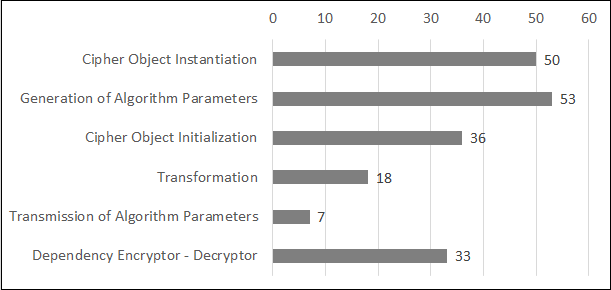
\includegraphics[width=0.85\textwidth]{TechnicalAspects}
\caption{Number of Issues Assigned to a Technical Aspects Main Category ($N = 219$)}
\label{fig:TechAspPlot}
\end{figure}

\par
% === Technical Aspects ===
As shown in figure \ref{fig:TechAspPlot}, the most common main categories in the first categorization round were \emph{Generation of Algorithm Parameters} and \emph{Cipher Object Instantiation}.
The most common subcategory was \emph{Key Derivation} with a total of 36 issues (16.4\%). This is not surprising as previous work has already shown that programmers struggle with key handling.
The set of issues referring to the key made up more than $\frac{1}{5}$ of all issues. This was only topped by the set of issues related to the various dependencies (27 \%).\\
Within the \emph{Cipher Object Instantiation} category, most issues referred to the encryption mode (18), padding (11) or the dependency between these properties (11).\\
The third most common main category was \emph{Cipher Object Initialization}. 
Most issues were assigned to its \emph{"Other"} subcategory.
They often refer to the default behavior of the \lstinline|init(...)| method if not all required properties were specified.\\
The fourth most common main category was \emph{Dependency Encryptor - Decryptor}.
The high prevalence of this category and the other dependency related subcategories implies that people lack knowledge about (symmetric) encryption in general.
The fact that the cipher objects for encryption and decryption must use the exact same algorithms and parameters is \emph{the} basic principle of symmetric encryption.\\
The other main categories and subcategories were not assigned that often.
You can find the complete list of categories and their frequencies of assignment in table \ref{tab:TechAspTab}.\\
\begin{table}[h]
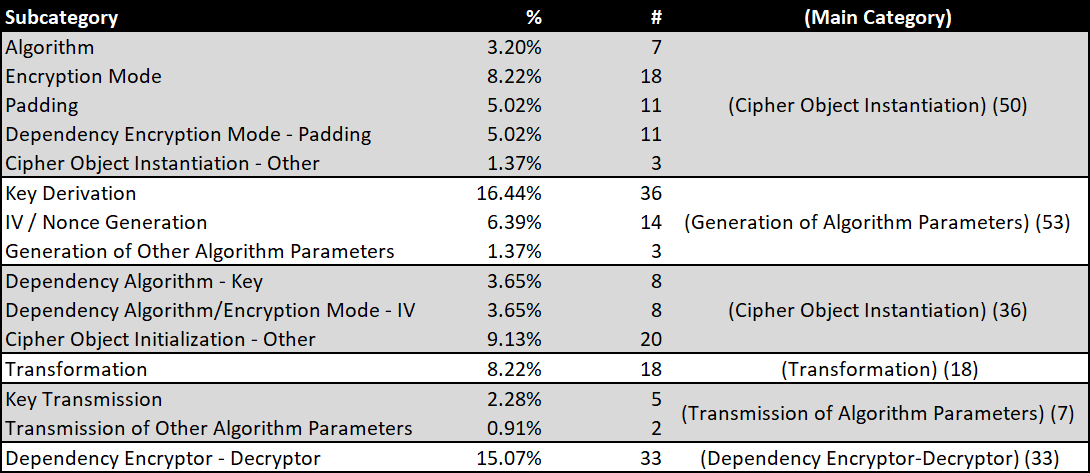
\includegraphics[width=1\textwidth]{TechAspTable}
\caption{Number of Issues Assigned to a Technical Aspect Subcategory ($N = 219$)}
\label{tab:TechAspTab}
\end{table}

% === Requirements ===
\par
Within the categories referring to requirements, \emph{Security} was the dominating category (46 records - 21\%).
This seems natural as this is what cryptography is all about.
Most issues were not mentioned in the question post.
They refer to security hints by people commenting or answering. 
Yet, there is massive under-reporting as our results from the security related analysis show (see section \ref{cha:ResSec}).\\
The other categories occurred much less often as you can see in figure \ref{fig:Req}
\begin{figure}[h]
\centering
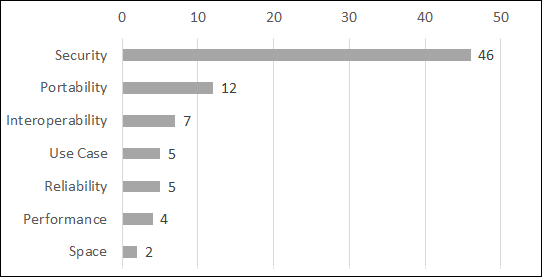
\includegraphics[width=0.8\textwidth]{Requirements}
\caption{Number of Issues Assigned to a Requirement Category ($N = 219$)}
\label{fig:Req}
\end{figure}

\newpage
\par
% === Doubly Classified Records ===
We observed the highest overlapping of categories for \emph{Generation of Algorithm Parameters} and \emph{Security} as well as 
\emph{Cipher Object Instantiation} and \emph{Security}. The heat map in figure \ref{fig:HeatMap} shows the relative overlapping of categories:
21\% of all posts classified as \emph{Generation of Algorithm Parameters} or \emph{Security} issue were assigned to both categories.
As we had less data for the other requirements categories, it is not surprising that we found much less overlapping for those.\\
\begin{figure}[h]
\centering
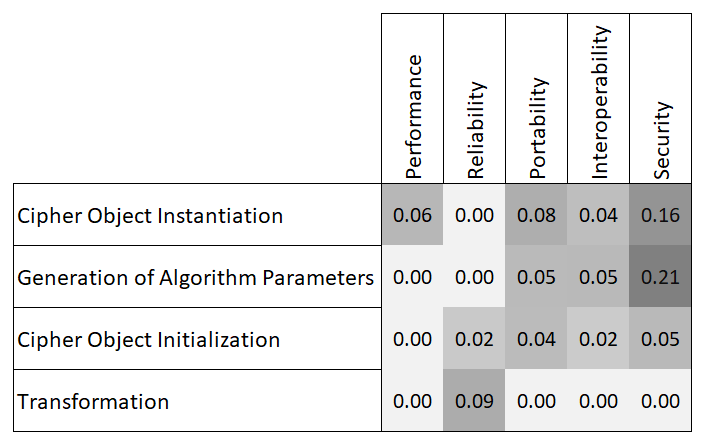
\includegraphics[width=0.8\textwidth]{HeatMap}
\caption{Relative Overlapping of Technical Aspects and Requirements Categories}
\label{fig:HeatMap}
\end{figure}



\newpage
% === Security ===
\section{Security Risks}
\label{cha:ResSec}
We manually checked 150 question,  84 answer posts, and related comments using our rule set.
We found a total of 331 security risks.
Most of them (249 - 75\%) stem from code snippets in question posts.
The text of question posts included only 38 security risks.
But we observed that the questions often did not contain much text.\\
We found 35 rule violations in answer related code snippets and 9 in related text.
We observed that some answers just fixed the functionality without improving its security.
The resulting code therefore "inherited" the security risks from the question.
Another common observation was that people correctly gave the advise that ECB was not considered save.
However, they suggested to use CBC which must not be used in client-server scenarios.
Such advise is therefore not safe, especially if we do not know in what kind of application the code section is used.\\
\begin{table}[h]
\centering
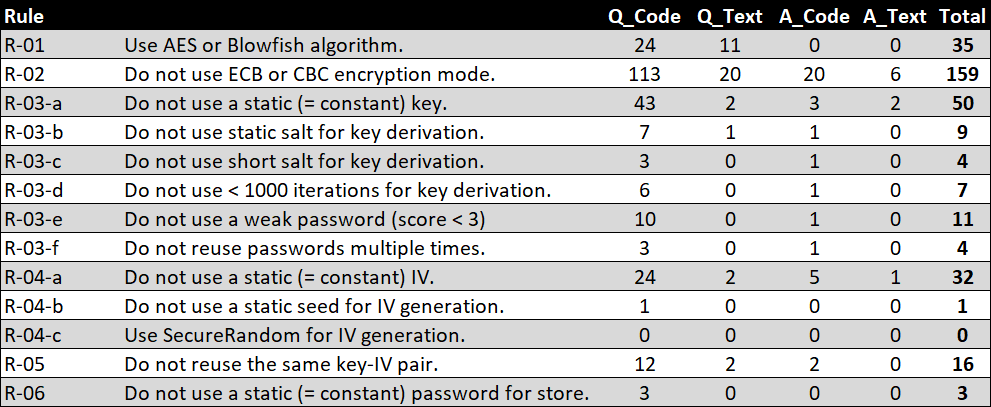
\includegraphics[width=1\textwidth]{SecTab}
\caption{Rule Violations per Check List}
\label{tab:SecRisk}
\end{table}
\par
% === Question Related Code
As we discovered most security risks in the question code, we focused on the evaluation of that check list.
The average question post contained 1.66 security risks in its code snippets.
We observed that the average for the most popular (and therefore older) posts (1.91) is slightly higher than the one for the newest posts (1.43).
24 question posts did not contain any security risk in their code snippets.\\
The most often violated rule was \emph{R-02: Do not use ECB or CBC encryption mode}. 
In more than 75\% of question posts, the original poster used one of these unsafe block cipher modes.
This is also due to ECB being the default encryption mode.
It is followed by the presence of constant keys (\emph{R-03-a}), unsafe password based key derivation procedures (\emph{R-03-b to R-03-f}, 29 recorded rule violations), and static
initialization vectors (\emph{R-04-a}).\\
Of course, the number of posts showing violations of \emph{R-01} is strictly related to the sample: 24 of our threads referred to DES or TripleDES encryption.
There were some code snippets in which the same key-IV pair was reused for several encryption operations.
This was related to using a constant key and a constant IV in most cases.


% === Documentation ===
\section{Documentation}
\label{cha:ResDoc}
We derived a total of 64 questions: 43 referring to documentation and 21 more general ones.
After checking the documentation, 10 questions remained unanswered and for 15 questions, we considered the answer as incomplete, unclear, or even misleading.\\

\subsection{Questions}
Our first observation regarding the questions was that there are twice as many JCA-specific questions as general ones.
Yet, the total priority of all "general" questions was much higher than the total priority of the specific ones even before correcting the priority for the security relevant ones.
This indicates one more time that programmers asking questions on Stack Overflow do not only lack knowledge about the JCA library but also about cryptography in general.\\

\par
The results from the first analysis gave us insight in what tasks and requirements programmers are struggling with.
The questions helped us to detect API related issues.
8 questions targeted a specific platform or were related to providers. 
2 of them were among the 3 most prioritized questions to documentation. 
As an example, the default behavior of a \lstinline|Cipher| object if not all required properties were specified during object instantiation or initialization also depends on the provider.
However, whether a provider is available or not and which provider is used by default depends on the platform.\\
Another 5 questions were related to method overloads. 

There are two methods that perform the data transformation and both of them are overloaded.
The methods for instantiation and initialization are overloaded as well.
\begin{table}[h]
\centering
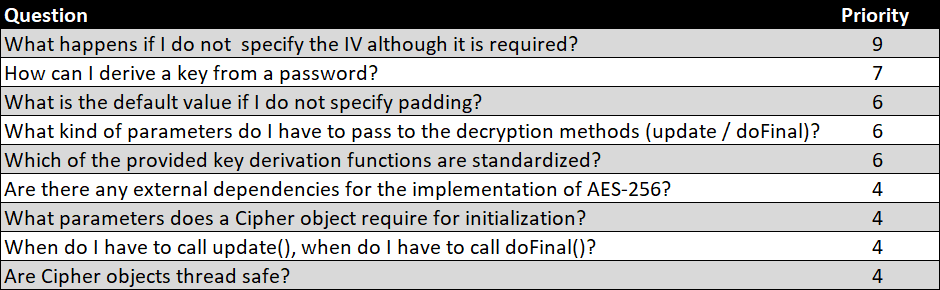
\includegraphics[width=1\textwidth]{QuestionsToDoc}
\caption{Top 9 JCA-Specific Questions}
\label{tab:Ques}
\end{table}

\subsection{Missing and Unclear Answers}
We were not able to find and answer to 3 JCA-specific and 7 general questions.
They all had a rather low priority (< 4).
The higher prevalence of unanswered general questions implies that JCA documentation does not provide (enough) links to trusted resources for general information about cryptography.\\
The following three unanswered questions represent documentation related issues:\\
\begin{itemize}
	\item \emph{How to specify PKCS\#7 padding in Java?}
					PKCS\#7 is a standardized padding for arbitrary block sizes that is supported by many cryptography libraries.
					JCA internally interprets PKCS\#5 padding as PKCS\#7 if it is required.
					However, this is not mentioned in the Standard Algorithm Name Specification nor in any other document that we examined.
					This might complicate the implementation of interoperability scenarios.
	\item \emph{What properties does AES-256 require?}
					There is a link to the official specifications for most algorithms in the Standard Algorithm Name Specification.
					However, for AES there is not.
					This is problematic since AES is one of only two symmetric encryption algorithms that are recommended.
	\item \emph{Which symmetric encryption algorithms are safe to use?}
					JCA documentation does not provide enough hints regarding security. 
\end{itemize}

\par
For 13 JCA specific questions and 2 more general ones, we considered the answers as not clear enough.
They often referred to method overloads. 
The documentation did not point out the differences clearly enough.
It often seemed like copy pasted.\\
Another common issue was that there is not any code example for some key scenarios (e.g using a \lstinline|KeyStore| or password based key derivation using PBKDF2).
The available ones often did not work due to some missing parts:
The code example for encryption did not show how the algorithm parameters were generated.



% === D I S C U S S I O N ===
\chapter {Conclusion and Future Work}
In this chapter, we first aim to answer our research questions based on our discussion from the previous chapter and add more context from related work.
We then present possible limitations of our study and suggest further research topics.
\colorbox{yellow}{ToDo}

\par{RQ 1}: \emph{What issues do programmers face when implementing symmetric encryption using Java Cryptography Architecture?}
Our study provided answers to this question from different perspectives.
If we think of \emph{tasks} that programmers are struggling with, most of them were struggling with key derivation and cipher object instantiation (especially specifying encryption mode and padding correctly).
The dependency from providers, unsafe default values, the existence of two kind of methods performing transformation, and the high amount of overloaded methods were the most common issues related to the \emph{library's design}.
But also the \emph{documentation} provided some obstacles:
It lacked working code examples, method overloads were documented too similarly, and there were not enough links to trusted sources for more general information about cryptography.\\
Of course, we should not forget the responsibility of programmers:
Our study added more evidence confirming the assumption that they lacked knowledge about cryptography.
However, we would like to extend it:
As the scope of our study was quiet limited, we excluded all threads that did not target it.
To collect our sample, we had to exclude 296 threads.
For each thread that (partly) belonged to our scope, there were two threads that did not.
Of those excluded threads, 138 (ca. 47\%) did either not refer to cryptography at all or they did not refer to the JCA library.
The large amount of threads containing non-cryptography-related issues only let us conclude that programmers do also lack knowledge about computer science in general.
We therefore should be aware that cryptography scenarios are implemented by programmers of all kind of backgrounds when we design a cryptography library.

\par{RQ 2}: \emph{What are common security risks in code and advises shared on Stack Overflow referring to the implementation of symmetric encryption scenarios Java Cryptography Architecture?}
\colorbox{yellow}{ToDo}\\

\par{RQ 3}: \emph{To what extent are those issues linked to missing or inadequate documentation?}
This research question is the most difficult one to answer.
We observed that most questions (>60\%) are clearly answered in the documentation.
We found relating information for almost 85\%.
Especially, the higher prioritized questions were clearly answered.
So we cannot blame insufficient documentation for the struggles of developers.
Yet, the documentation could be improved.
It should provide more (working) code examples, security hints, and links to trusted resources for more information about cryptography.
In the API documentation, the method overloads should be documented more specifically.
\colorbox{yellow}{ToDo}\\


\section{Limitations and Future Work}
As this project followed a qualitative approach performing an in-depth analysis, it is reasonable to have a limited scope.
Future work must extend it by examining more use cases and libraries.\\

\par
When it comes to the methodical approach, one threat to validity is that the population of Stack Overflow threads matching the criteria cannot be described exactly.
There is no guarantee that the used queries returned all posts referring to symmetric encryption using the targeted libraries.
However, this is not possible with a finite set of queries as you cannot know which posts you did not find.
This circumstance implies that the results must be verified with further investigations.\\
Also, the sample cannot be considered as representative for the posts returned by the defined queries as a lot of posts (ca. $\frac{2}{3}$) were excluded because they did not match the predefined criteria.
The high ratio of posts not referring to cryptography and not referring to the library implies that people do not only struggle with cryptography when implementing a cryptography scenario. %ToDo: Herausfinden, wie viele Posts!
This observation reveals new research areas and questions. 
But it also complicates the design of cryptography APIs as it should satisfy a security expert equally as a "newbie".\\

 \section{Conclusion}


% === Future Work ===
% Examine other use cases: asymmetric encryption, message authentication, hashing, ...
% Examine more libraries
% Findings from research must also be taken into account in the development of new libraries or in the refactoring of existing ones



% === A N L E I T U N G   Z U   W I S S E N S C H A F T L I C H E M   A R B E I T E N
\chapter {Anleitung zu wissenschaftlichen Arbeiten}
\label{cha:AWI}
This chapter describes the methodical approach of qualitative content analysis according Mayring \cite{mayring2015}.
Each section refers to a work step of the processing scheme which is first explained generally and then applied to the derivation of issues from Stack Overflow threads, see chapter \ref{cha:MetIssues}.\\
Please note that the aim of this chapter is to specify the processing scheme more precisely.
All kind of justification can be found in the methodology section of this thesis.

%ToDo: Citations?
\section{Presenting the Sample}
Defining and presenting the sample is the first step in qualitative content analysis: 
We describe the population, the context of its creation and its formal characteristics as well as the sampling process.

\subsection{Population}
Stack Overflow is one of the most popular online forums for programmers.
According to the developer survey from 2020, about 50 million people visit the platform per month.
Approximately 50\% of them are either professional developers or university-level students \cite{stackoverflow2020}.
As we only want to examine threads that refer to the implementation of symmetric encryption using the Java Cryptography Architecture library,
we define our population as the set of posts returned by at least one of the following queries:
\newpage
\begin{itemize}
	\item \lstinline|[java] Cipher.getInstance("AES")|
	\item \lstinline|[java] Cipher.getInstance("DESede")|
	\item \lstinline|[java] Cipher.getInstance("DES") --DESede|
\end{itemize}
\par
We do not know a lot about the context of our population.
Especially, we do not know anything about the people writing the posts and comments.
Based on the findings by Nadi \etal \cite{nadi2016}, we assume that the people asking questions are professional developers (industrial or freelance), researchers or students who must implement a symmetric encryption scenario either for work or education.
However, their backgrounds regarding experience with Java as a programming language or cryptography are very heterogeneous.
In Nadi \etal's survey, the test persons declared that they "spend at least several hours reading through online resources" (2016, \cite{nadi2016}, p. 938) before asking on Stack Overflow.\\
\par
All material is available online on Stack Overflow.
It reflects a conversation between one or several users.
For each post, we can see the username of the author as well as the date and time of its creation.
Some posts have been edited after their creation.
In that case, we can see the username and the date of the last edit.
However, we cannot reproduce what has been changed.
Sometimes, persons also delete their posts or comments.
Such posts are not visible anymore.


\subsection{Sampling Process}
Based on the total number of posts returned by the queries (3828) we calculated that 150 threads should be enough to satisfy our requirements of a confidence level of at least 95 \% and a margin of error below 10\%.
Next, we computed the number of threads per query proportionally to the number of posts it returned.
Finally, we selected the threads for our sample.
We picked half of the sample from the "newest" threads which was determined by the creation date of the question post.
We took the other half from the most popular ones based on the view count of the question.
Also, we only selected threads that addressed at least one issue within our scope.
Other posts were excluded for at least one of the following reasons: \colorbox{yellow}{ToDo: C\# Beispiele austauschen}
\begin{itemize}
	\item \textbf{too general}: posts referring to cryptographic concepts or cyber security in general rather than the targeted API\\ 
			\emph{Example: \href{https://stackoverflow.com/questions/939040/when-will-c-sharp-aes-algorithm-be-fips-compliant}{When will C\# AES algorithm be FIPS compliant?}}

	\item \textbf{does not refer to cryptography}: issues occurring in a non-cryptographic context, i.e. establishing a network connection or file access\\
			\emph{Example: \href{https://stackoverflow.com/questions/1755259/syntax-error-on-token-expected-after-this-token}{Syntax error}}

	\item \textbf{does not refer to symmetric encryption}: posts referring to other cryptographic concepts such as asymmetric encryption or hashing\\
			\emph{Example: \href{https://stackoverflow.com/questions/66941359/rsa-decryption-fails}{RSA decryption (fails)}} 

	\item \textbf{does not refer to JCA}: issues occurring during a symmetric encryption scenario but which are not due to Java Cryptography Architecture.
				Such issues can refer to another library (e.g. BouncyCastle) or to some other aspect such as character encoding.\\
				\emph{Example: \href{https://stackoverflow.com/questions/5641326/256bit-aes-cbc-pkcs5padding-with-bouncy-castle}{256bit AES/CBC/PKCS5Padding with Bouncy Castle}}

	\item \textbf{does not refer to targeted algorithm}: posts referring to other algorithms than the targeted ones\\
			\emph{Example: \href{https://stackoverflow.com/questions/68772573/how-to-use-password-with-pbekeyspec-hash}{how to use password with \lstinline|PBEKeySpec| hash}}

	\item \textbf{looking for an equivalent} or \textbf{interoperability issue}:  looking for equivalents / counterparts in different programming languages\\
			\emph{Example: \href{https://stackoverflow.com/questions/64902430/change-rijndael-decryption-logic-from-c-sharp-to-python}{Change Rijndael decryption logic from C\# to Python}} 

	\item \textbf{negative votes} or \textbf{closed}: posts of poor quality

	\item \textbf{academic}: posts with a different focus than obstacles when using the API

	\item \textbf{duplicate}: Duplicates are often left unanswered (or only answered with the reference to a similar post). For posts belonging to the "most popular" category, we included a duplicate if it had more views than the original.
\end{itemize}


\newpage
\section{Specific Research Questions}
The second step of qualitative content analysis is to describe precisely what the aim of the interpretation is.
We must provide a set of well defined research questions that are theoretically differentiated.\\

\par
The aim of our first analysis was to find an answer to the first research question of the thesis:
\emph{What issues do programmers face when implementing symmetric encryption using Java Cryptography Architecture?}
A (piece of) software must meet various requirements. 
\colorbox{yellow}{ToDo: Consult Sommerville}


\section{Processing Scheme for Interpretation}
Summarizing:
The coding unit of this first round of analysis was a single word (e.g. an error message).
The context unit was an entire post or a comment.\\


\section{Evaluation of Specific Quality Criteria}

%ToDo: Kommt in "Anleitung zu wissenschaftlichem Arbeiten"
%To verify intercoder reliabilty, 15 posts per library (10\%) were randomly chosen and reviewed by two colleagues who were not involved in the project.
%After a quick introduction to the categories and the procedure, they followed the same scheme as just described.
%As the records were formed inductively, there was no point in verifying them.
%However, the set of categories assigned to a thread were compared.



% === B I B L I O G R A P H Y ===
\bibliography{thesis}
\bibliographystyle{plain}

% === A C K N O W L E D G E M E N T S ===
\chapter{Acknowledgments}



% === A P P E N D I X ===
\chapter{Appendix}
\section*{A \hspace{5mm} Sample and Analysis Related Data}

%END Doc
%-------------------------------------------------------



\end{document}